
\documentclass[12pt]{amsart}
\usepackage{geometry} % see geometry.pdf on how to lay out the page. There's lots.
\usepackage{epsfig}
\usepackage{graphicx}
\usepackage{subfig}

\geometry{a4paper} % or letter or a5paper or ... etc
% \geometry{landscape} % rotated page geometry

% See the ``Article customise'' template for come common customisations

\title{ISYE 6663 Project Report}
\author{Brant Calloway, John Rogers}
\date{} % delete this line to display the current date

%%% BEGIN DOCUMENT
\begin{document}

\maketitle
%\tableofcontents

\section{Project Implementation}
For our project, we implemented the Gradient Descent method, two versions of Conjugate Gradient method (Fletcher-Reeves and Polak-Ribiere), the Quasi-Newton BFGS method, and the limited memory BFGS method. In order to test our algorithms, we implemented four functions with known properties.  These were the Rosenbrock function, the Trigonometric function, Wood function, and a large quadratic function.  Exact line search was used with the quadratic problem, and a strong Wolfe-Powell inexact line search was used on all of the problems.  

\subsection{Optimization Routine Implementation}

Both of the conjugate gradient methods (CGFR and CGPR) often did not converge to sufficient precision on some of the harder nonlinear problems.  This is due to round off errors from finite precision computer arithmetic as well as local quadratic approximation of the function changes for nonlinear problems as we move from one step to the next.  Each of the search directions explored by CG is Q-Conjugate to the prior search directions.  Since we are using an inexact line search procedure, one search along this direction may not be sufficient to reach the global minimum.  To combat this shortcoming, we reset to a gradient descent step whenever two consecutive gradients are not sufficiently orthogonal, as was suggested in the textbook.  This effectively resets the conjugate-gradient method to allow it to minimize along all search directions again.

The L-BFGS quasi newton optimization algorithm was implemented with a variable amount of memory storage.  Our original implementation had a fixed history of 5, but we chose to implement variable history to perform an analysis of how the history size affects the algorithm performance.  Our expectation is that when more history is added, the performance might degrade on some of the nonlinear problems as the Hessian approximation 

\subsection{Test Function Implementation}

Another issue that we had was in testing the Trigonometric function.  We had major concerns that we had implemented the function wrong or not gotten the gradient correct.  Finally, we found that from the starting point given($xo = (1/n, 1/n,\hdots,1/n)$) in the notes, there is a local minimum that occurs between that starting point and what the notes give as the correct solution $x* = (0,0,\hdots,0)$.  To further illustrate the point, here are the graphs for the trigonometric function with n=1 in figure~\ref{fig:2d-trig} and n=2 in figure~\ref{fig:3d-trig}.  We can see that for n=1, there is a local minimum close to 0.927 which is where our each of our algorithms terminate (and further notice that this occurs between x*=0 and xo = 1/1 = 1. Similarly, for n=2, although slightly more difficult to see in the graph, we find a local minimum at x = (0.243, 0.613) rather than at x* = (0,0).  In our results section, we will present the convergence to this local minimum, plus the convergence to the true global minimum from a different starting point.

We also implemented the Wood function from the test problems sheet and we run on the Rosenbrock function which was provided.  In addition, we prepared a large quadratic function primarily to test the exact line search performance compared to inexact line search.  The Rosenbrock function was tried with multiple sizes up to 20 dimensions, as was the Trigonometric function.

\begin{figure}[thpb]
\centering
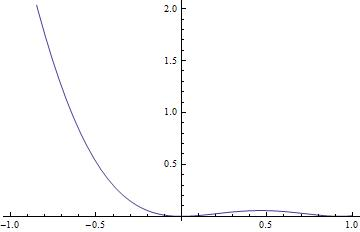
\includegraphics[scale=0.60]{images/2dtrig.jpg}
\caption{The trigonometric function, shown in 1 dimension.  The optimization routine gets stuck in a local minimum.}
\label{fig:2d-trig}
\end{figure}

\begin{figure}[thpb]
\centering
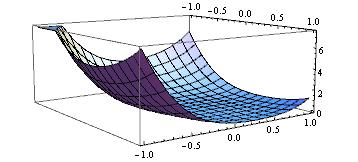
\includegraphics[scale=0.60]{images/3dtrig.jpg}
\caption{The trigonometric function, shown with 2 dimensions.  The optimization routine gets stuck in a local minimum.}
\label{fig:3d-trig}
\end{figure}

\section{Results}
The number of iterations and cpu time are compared between each of the tested algorithms on each of the test problems.  In addition, the number of restarts are presented for the CG methods.  The gradient descent algorithm is usually only able to reach a lower precision than the other routines due to its inefficiency with poorly conditioned problems. 

\subsection{Quadratic Results}

The optimization routines were first tried on a quadratic problem of the form $min x^T A x - b^T x $.  The matrix $A$ was generated by the rand function in Matlab and made to be positive definite by computing $A^T A$.  The vector $b$ was also computed using the rand function.  The results for exact line search can be seen in table \ref{table_exact_quad}.  Comparing these results to table \ref{table_inexact_quad}, we see that the gradient descent routine achieves the desired precision in exactly the same number of iterations, though exact line search is much quicker than inexact line search for CPU time.  Further inspection led us to realize that the inexact line search routine was generating the exact same $\alpha_k$ as the exact line search routine.  The difference in CPU time is due to the simplicity in the exact line search -- gradient descent spends a lot of CPU cycles on inexact line search.  A few other notable differences are that the conjugate gradient methods terminate in about 20 iterations and don't require restarts when using exact line search.  When they use inexact line search, more iterations are necessary and restarts are also used multiple times.  Our implementation of strong Wolfe-Powell appears to generate exact line search results when the gradients are parallel to the search directions, so since the CG methods do not use gradient directions the two line search routines generate different $\alpha_k$.  The BFGS routine terminates in 21 iterations, which makes sense because after the first 20 iterations the Hessian approximation is exact and the final step is a Newton step.  On a quadratic function, this results in the solution being reached in only one more iteration.  

\begin{table}
\caption{Experimental Results - Quadratic Function, exact line search, 20 dimensional, $\eta=1e-4$}
\label{table_exact_quad}
\begin{center}
\begin{tabular}{|c||c||c||c||c|}
\hline
Algorithm & Iterations & CPU-Time & Restarts & Notes\\
\hline
GD & 61368 & 15.776 & 0 & \\
\hline
CG-FR & 26 & 0.110 & 0 & \\
\hline
CG-PR & 26 & 0.078 & 0 & \\
\hline
BFGS & 21 & 0.081& 0 & \\
\hline
L-BFGS-5 & 496 & 0.427 & 0 &\\
\hline
L-BFGS-7 & 392 & 0.537 & 0 &\\
\hline
L-BFGS-9 & 284 & 0.482 & 0 &\\
\hline
L-BFGS-11 & 321 & 0.804 & 0 &\\
\hline
\end{tabular}
\end{center}
\end{table}


\begin{table}
\caption{Experimental Results - Quadratic Function, inexact line search, 20 dimensional, $\eta=1e-4$}
\label{table_inexact_quad}
\begin{center}
\begin{tabular}{|c||c||c||c||c|}
\hline
Algorithm & Iterations & CPU-Time & Restarts & Notes\\
\hline
GD & 61368 & 41.357 & 0 & \\
\hline
CG-FR & 77 & 0.157 & 5 & \\
\hline
CG-PR & 202 & 0.238 & 14 & \\
\hline
BFGS & 24 & 0.140& 0 & \\
\hline
L-BFGS-5 & 310 & 0.490 & 0 &\\
\hline
L-BFGS-7 & 330 & 0.648 & 0 &\\
\hline
L-BFGS-9 & 413 & 0.899 & 0 &\\
\hline
L-BFGS-11 & 268 & 0.771& 0 &\\
\hline
\end{tabular}
\end{center}
\end{table}

\subsection{Trigonometric Results}
\begin{table}
\caption{Experimental Results - Trigonometric Function 10 dimensional, 1/n starting point, $\eta=1e-8$}
\label{results_table}
\begin{center}
\begin{tabular}{|c||c||c||c||c|}
\hline
Algorithm & Iterations & CPU-Time & Restarts & Notes\\
\hline
GD & 167 & 0.087 & 0 & Stuck\\
\hline
CG-FR & 54 & .150 & 15 & Stuck\\
\hline
CG-PR & 49 & .152 & 17 & Stuck\\
\hline
BFGS & 24 & .139 & 0 & Stuck\\
\hline
L-BFGS-5 & 59 & 0.181 & 0 & Stuck\\
\hline
L-BFGS-7 & 66 & 0.196 & 0 & Stuck\\
\hline
L-BFGS-9 & 77 & 0.24 & 0 & Stuck \\
\hline
L-BFGS-11 & 80 & 0.274 & 0 & Stuck\\
\hline
\end{tabular}
\end{center}
\end{table}
\begin{table}
\caption{Experimental Results - Trigonometric Function, 40 dimensional, starting point 1/(10n), $\eta=1e-12$}
\label{results_table}
\begin{center}
\begin{tabular}{|c||c||c||c||c|}
\hline
Algorithm & Iterations & CPU-Time & Restarts & Notes\\
\hline
GD & 6 & 0.0144 & 0 & \\
\hline
CG-FR & 5 & 0.0492 & 3 & \\
\hline
CG-PR & 5 & 0.048 & 3 & \\
\hline
BFGS & 11 & 0.682 & 0 & \\
\hline
L-BFGS-5 & 14 & 0.0896 & 0 &\\
\hline
L-BFGS-7 & 12 & 0.089 & 0 &\\
\hline
L-BFGS-9 & 13 & 0.117 & 0 &\\
\hline
L-BFGS-11 & 13 & 0.129 & 0 &\\
\hline
\end{tabular}
\end{center}
\end{table}

\subsection{Wood Results}

\begin{table}
\caption{Experimental Results - Wood Function, $\eta=1e-10$}
\label{results_table}
\begin{center}
\begin{tabular}{|c||c||c||c||c|}
\hline
Algorithm & Iterations & CPU-Time & Restarts & Notes\\
\hline
GD & 6707 & 1.64 & 0 & \\
\hline
CG-FR & 115 & 0.163 & 43 & \\
\hline
CG-PR & 139 & 0.172 & 55 & \\
\hline
BFGS & 62 & 0.165 & 0 & \\
\hline
L-BFGS-5 & 111 & 0.202 & 0 &\\
\hline
L-BFGS-7 & 141 & 0.232 & 0 &\\
\hline
L-BFGS-9 & 152 & 0.271 & 0 &\\
\hline
L-BFGS-11 & 170 & 0.312 & 0 &\\
\hline
\end{tabular}
\end{center}
\end{table}

\subsection{Rosenbrock Results}
\begin{table}
\caption{Experimental Results - Rosenbrock Function 6 dimensional, $\eta=1e-10$}
\label{results_table}
\begin{center}
\begin{tabular}{|c||c||c||c||c|}
\hline
Algorithm & Iterations & CPU-Time & Restarts & Notes\\
\hline
GD & $>14718$ & $>4sec$ & 0 & $\eta=1e-2$\\
\hline
CG-FR & 371 & 0.157 & 65 & \\
\hline
CG-PR & 387 & 0.231 & 60 & \\
\hline
BFGS & 116 & 0.172 & 0 & \\
\hline
L-BFGS-5 & 266 & 0.287 & 0 &\\
\hline
L-BFGS-7 & 327 & 0.343 & 0 &\\
\hline
L-BFGS-9 & 372 & 0.413 & 0 &\\
\hline
L-BFGS-11 & 449 & 0.561 & 0 &\\
\hline
\end{tabular}
\end{center}
\end{table}

\begin{table}
\caption{Experimental Results - Rosenbrock Function 8 dimensional, $\eta=1e-10$}
\label{results_table}
\begin{center}
\begin{tabular}{|c||c||c||c||c|}
\hline
Algorithm & Iterations & CPU-Time & Restarts & Notes\\
\hline
GD & $>14508$ & $>3.86$& 0  & $\eta=1e-2$ \\
\hline
CG-FR & 1120 & 0.353 & 146 & \\
\hline
CG-PR & 1186 & 0.465 & 150 & \\
\hline
BFGS & 258 & 0.245 & 0 & \\
\hline
L-BFGS-5 & 572 & 0.444 & 0 &\\
\hline
L-BFGS-7 & 762 & 0.675 & 0 &\\
\hline
L-BFGS-9 & 992 & 0.987 & 0 &\\
\hline
L-BFGS-11 & 1062 & 1.24 & 0 &\\
\hline
\end{tabular}
\end{center}
\end{table}

\begin{table}
\caption{Experimental Results - Rosenbrock Function 10 dimensional, $\eta=1e-10$}
\label{results_table}
\begin{center}
\begin{tabular}{|c||c||c||c||c|}
\hline
Algorithm & Iterations & CPU-Time & Restarts & Notes\\
\hline
GD & $>14508$ & $>3.875$ & 0 & $\eta=1e-2$ \\
\hline
CG-FR & 3543 & 1.031 & 358 & \\
\hline
CG-PR & 3465 & 1.105 & 384 & \\
\hline
BFGS & 589 & 0.373 & 0 & \\
\hline
L-BFGS-5 & 1286 & 0.922 & 0 &\\
\hline
L-BFGS-7 & 1888 & 1.65 & 0 &\\
\hline
L-BFGS-9 & 2250 & 2.458 & 0 &\\
\hline
L-BFGS-11 & 3383 & 4.59 & 0 &\\
\hline
\end{tabular}
\end{center}
\end{table}

\begin{table}
\caption{Experimental Results - Rosenbrock Function 20 dimensional, $\eta=1e-5$}
\label{results_table}
\begin{center}
\begin{tabular}{|c||c||c||c||c|}
\hline
Algorithm & Iterations & CPU-Time & Restarts & Notes\\
\hline
GD & $>14508$ & $>3.9$ & 0 & $\eta=1e-2$\\
\hline
CG-FR & 2522 & 0.818 & 243 & \\
\hline
CG-PR & 2713 & 0.887 & 262 & \\
\hline
BFGS & 2184 & 1.18 & 0 & \\
\hline
L-BFGS-5 & 10124 & 8.42 & 0 &\\
\hline
L-BFGS-7 & 10625 & 12.8 & 0 &\\
\hline
L-BFGS-9 & 14011 & 23.4 & 0 &\\
\hline
L-BFGS-11 & 14030 & 32.6 & 0 &\\
\hline
\end{tabular}
\end{center}
\end{table}



Nothing Yet...


\section{Conclusion}
The main thing that we learned in working on this project was that between almost any of the methods, there are tradeoffs.  

Before we implemented restarts in the CG methods, the Polak-Ribiere Conjugate Gradient method performed much better than the Fletcher-Reeves method which we expected.  When we implemented restarts, both methods improved; however, the CGFR improved so much more that it seems to now be more effective than the CGPR on our test problems.  

The Gradient Descent algorithm was usually too slow to run to the same convergence as the more sophisticated optimization routines were able to achieve.  On the 20 dimensional Rosenbrock function, the BFGS routine was about to achieve 8 more decimal points of accuracy than the GD with far less computation.  

The BFGS method took the fewest number of iterations to converge.  However, it was not always the fastest.  And the limited memory BFGS method took more iterations to complete, but was sometimes faster than the BFGS method.  Further, the performance of the limited BFGS method depended strongly upon the number of vectors to remember.  Remarkably, we found an instance where we increased the number of vectors to remember and also increased the number of iterations to get to the solution.

\end{document}